\subchapter{Toolchain optimization}{Get the best cross-compiling
toolchain for your application and system}

The goal of this lab is to find the best toolchain for your application,
in terms of performance and code size. Smaller code can be faster to
load, and save time when using in an initramfs (when the whole
filesystem is loaded at once in RAM).

In this lab, we will see how to test an alternative toolchain, measuring:
\begin{itemize}
 \item Application execution time
 \item Application and total filesystem size
\end{itemize}

\section{Measuring application execution time}

At this stage, measuring the total system boot time is not accurate
enough. We need to time the execution of the application more precisely.

Hence, we will call the \code{ffmpeg} player directly from the command
line and temporarily apply a patch that will make \code{ffmpeg}
exit after processing the first frame.

To achieve this:
\begin{itemize}
\item Temporarily replace the previously applied ffmpeg patch
by \code{0001-ffmpeg-exit-after-first-frame.patch} found in
\code{~/boot-time-labs/rootfs/data/}.
\item Edit the \code{S50playvideo} script to comment out the line
starting \code{ffmpeg} automatically. We don't want \code{ffmpeg} to run
automatically at this stage, because otherwise when won't be able to
time its first execution through the \code{time} command and then
compare with the second time it is executed, to have an measurement of
the \code{ffmpeg} loading time.
\end{itemize}

Now, rebuild the root filesystem:
\begin{verbatim}
make ffmpeg-dirclean
make
\end{verbatim}

Let's measure the total root filesystem size and the size of the
\code{ffmpeg} executable:

\begin{verbatim}
ls -l output/images/rootfs.tar
tar tvf output/images/rootfs.tar ./usr/bin/ffmpeg
\end{verbatim}

Write these two numbers in the first row of the \code{~/boot-time-labs/results/toochain-size-tests.ods}
spreadsheet:

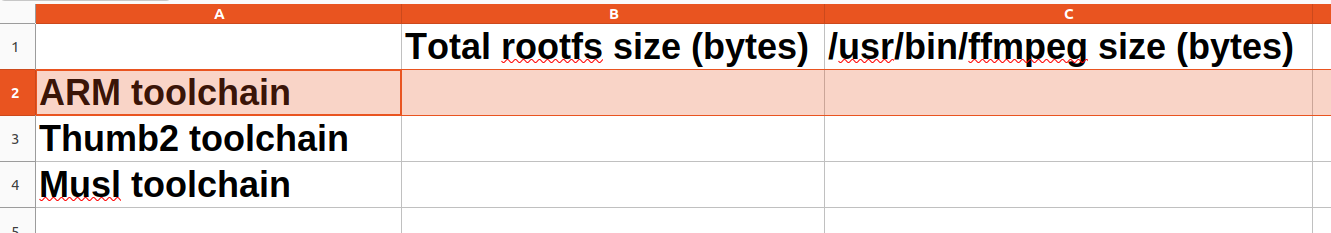
\includegraphics[width=0.7\textwidth]{labs/boot-time-toolchain/toolchain-size-tests.png}

Reflash the root filesystem on the SD card and reboot your board.
On the serial console, log in and run the video player through the
\code{time} command (copying and pasting the command from these
instructions or from the \code{/etc/init.d/S50playvideo} file:

\begin{verbatim}
time ffmpeg -f video4linux2 -video_size 544x288 -input_format mjpeg \
-i /dev/video0 -pix_fmt rgb565le -f fbdev /dev/fb0
\end{verbatim}

Note that we removed \code{-t 10}. It's no longer needed to stop after
10 seconds as we stop after decoding the first frame.

Run the experiment 3 times and write down your first results in the first
row of the \code{boot-time-labs/results/toochain-time-tests.ods} spreadsheet:
filling the \code{total<n>}\code{user<n>} and \code{sys<n>} columns):

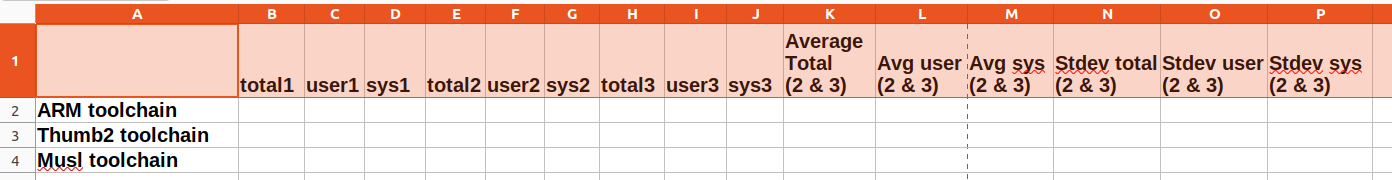
\includegraphics[width=\textwidth]{labs/boot-time-toolchain/toolchain-time-tests.png}

After the first run, the program and its shared libraries are now in the
file cache. Lets run the command two more times and write down (in the
\code{2} and \code{3} columns) how fast it can run in this ideal case.

\section{Switching to a Thumb2 toolchain}

Now, let's modify the Buildroot toolchain, so that it generates {\em
Thumb2} code (instead of {\em ARM}) by default.

Before we switch, let's make a backup of the \code{buildroot} directory,
in case results are disappointing and we wish to revert the changes without
having to go through a full build again. In our particular case, we will
start the next lab using this backup, waiting for the new build to be
complete.

In case you didn't know, a time and disk space efficient way to do this is by using the
\code{cp -al} command, which uses hard links instead of making new copies
of each file:

\begin{verbatim}
cd ..
cp -al buildroot buildroot-arm
\end{verbatim}

You can then check that the files correspond to the same inode:
\begin{verbatim}
ls -i buildroot/Makefile buildroot-arm/Makefile
\end{verbatim}

Back to the \code{buildroot} directory, run \code{make menuconfig}, and
in \code{Target options}, set \code{ARM instruction set} to
\code{Thumb2}.

Save the changes and run the full toolchain and root filesystem build
again:

\begin{verbatim}
make clean
make
\end{verbatim}

This is probably going to run for at least 30 minutes. In the meantime,
start working on the next lab.

When the build is over:
\begin{itemize}
\item Measure the new root filesystem archive and \code{ffmpeg}
executable size, write it down in the table, and compute the difference
percentages vs. the ARM code.
\item Update the SD card with the new filesystem, run the same time
measurements, and write down the results to compare them with the ARM
ones. You can also add the percentage difference.
\end{itemize}

So, was it a good choice to switch to {\em Thumb2}? Where there any size
and performance benefits?

Don't hesitate to show your results to your instructor.

\section{Test the musl C library}

The last thing to try in this lab is using a toolchain with the {\em
Musl} C library, instead of {\em uClibc}, which is the C library that
Buildroot uses by default.

Once again, keep a copy your current Buildroot directory:
\begin{verbatim}
cd ..
cp -al buildroot buildroot-thumb2
\end{verbatim}

Back to the \code{buildroot} directory, run \code{make menuconfig}, and
in \code{Toolchain}, set \code{C library} to to \code{musl}.

Save, run \code{make clean} and build the root filesystem once again.

Once again, write down the two sizes and measure \code{ffmpeg} execution
time.

Now, what the best combination? {\em ARM} or {\em Thumb2},
{\em uClibc} or {\em Musl}?

If you have the same size and performance between {\em uClibc} or {\em
Musl}, its better to choose the latter, as according to the slides, it
will allow to generate smaller static executables (we will try that
in later instructions). Another reason is that the {\em Musl} library
has a more liberal license, making it easier to ship static executables.

\section{Generate a Buildroot SDK to rebuild faster}

Choose Buildroot configuration that worked best for you, renaming
the directory to \code{buildroot} if that was not the last one you
tried.

With Buildroot, it's frequent to need to run \code{make clean} and
thus make a full rebuild, typically after configuration changes.
As you've seen, such rebuilds are expensive with our Buildroot
configuration that builds the toolchain too.

Now that we have finalized our toolchain, let's have Buildroot generate
an SDK that we won't have to build from scratch every time we need a
full rebuild. In the below instructions, you assume that you chose a
{\em Musl} toolchain:

\begin{verbatim}
make sdk
cd ~/boot-time-labs/rootfs
tar xf buildroot/output/images/arm-buildroot-linux-musleabihf_sdk-buildroot.tar.gz
cd arm-buildroot-linux-musleabihf_sdk-buildroot
./relocate-sdk.sh
\end{verbatim}

Let's then configure Buildroot to use this new toolchain:
\begin{verbatim}
cd ../buildroot/
make menuconfig
\end{verbatim}

In the \code{Toolchain} menu:
\begin{itemize}
\item Set \code{Toolchain type} to \code{External toolchain}
\item Set \code{Toolchain} to \code{Custom toolchain}
\item Set \code{Toolchain origin} to \code{Pre-installed toolchain}
\item Set \code{Toolchain path} to\\
      \code{/home/<user>/boot-time-labs/rootfs/arm-buildroot-linux-musleabihf_sdk-buildroot}
      (replace \code{<user>} by your actual user name)
\item Set \code{External toolchain gcc version} to \code{11.x}
\item Set \code{External toolchain kernel headers series} to \code{5.16.x or later}
\item Set \code{External toolchain C library} to \code{musl (experimental)}
\end{itemize}

Now test that your settings are correct:

\begin{verbatim}
make clean
make
\end{verbatim}
